% Triton kernel Roofline scatter plot
% Compile: pdflatex kernel_roofline.tex
% Inline:  % Triton kernel Roofline scatter plot
% Compile: pdflatex kernel_roofline.tex
% Inline:  % Triton kernel Roofline scatter plot
% Compile: pdflatex kernel_roofline.tex
% Inline:  % Triton kernel Roofline scatter plot
% Compile: pdflatex kernel_roofline.tex
% Inline:  \input{figures/kernel_roofline.tex}
%
% 数据来源:
%   profile_v2_h800.md   (forward-only)        — Roofline 段 + Actual TFLOPS 列
%   profile_bwd_h800.md  (forward + backward)  — Roofline 段 + Actual TFLOPS 列
% 测试硬件: NVIDIA H800 PCIe
%   - BF16 Tensor Core peak: 756 TFLOPS (dense, 厂商标称)
%   - HBM3 sustained BW    : ~1.26 TB/s (~63% of 2.0 TB/s theoretical)
%   - Ridge point          : 756 / 1.26 ≈ 600 FLOPs/byte
%
% 设计要点:
%   - log-log 双对数: AI 跨 0.7-770 (3 数量级), TFLOPS 跨 0.007-96 (4 数量级)
%   - Memory roof (蓝色斜线, slope=BW): y = 1.26 * x, 适用于 x < 600
%   - Compute roof (红色水平线): y = 756, 适用于 x ≥ 600
%   - Ridge 灰色虚线: AI = 600 处屋脊
%   - AI=100 绿色点线: md 经验阈值 (memory-bound 实用判定)
%   - 8 kernels × 2 workloads: 蓝圆 = forward-only, 橙三角 = forward+backward
%   - 同 kernel 的 fwd / fwd+bwd 用细灰线连接, 线长直观显示 backward 性能衰减
%   - 关键 kernel 名称直接标注在点旁; 反面案例 linear_ce 突出标红
\documentclass[tikz,border=10pt]{standalone}
\usepackage{pgfplots}
\usepackage{amsmath}
\pgfplotsset{compat=1.18}

\begin{document}
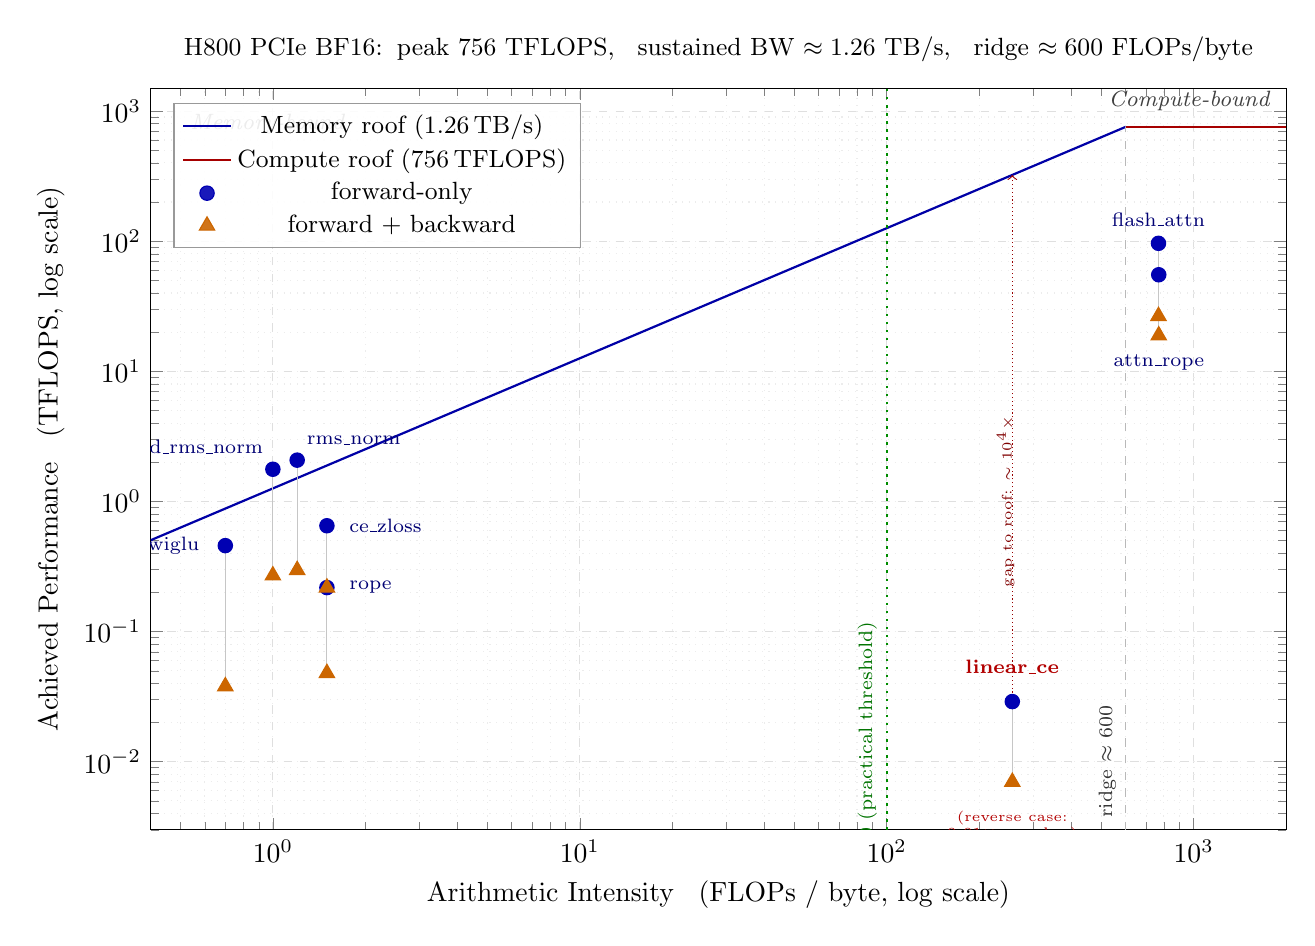
\begin{tikzpicture}
\begin{axis}[
    width=16cm,
    height=11cm,
    xmode=log, ymode=log,
    log basis x=10, log basis y=10,
    xmin=0.4, xmax=2000,
    ymin=0.003, ymax=1500,
    xlabel={Arithmetic Intensity \;\;(FLOPs / byte, log scale)},
    ylabel={Achieved Performance \;\;(TFLOPS, log scale)},
    grid=both,
    major grid style={dashed, gray!25},
    minor grid style={dotted, gray!15},
    legend style={
        at={(0.02,0.98)}, anchor=north west,
        font=\small, draw=black!40, fill=white, fill opacity=0.9,
        text opacity=1
    },
    title style={font=\small},
    title={H800 PCIe BF16:\;\;peak $756$ TFLOPS,\;\; sustained BW $\approx 1.26$ TB/s,\;\; ridge $\approx 600$ FLOPs/byte},
]

% =========================================================
% Roofline ceilings
% =========================================================
% Memory roof: P = BW * AI = 1.26 * x (TFLOPS = TB/s * FLOPs/byte)
% draws from x=0.4 up to ridge x=600, where y = 1.26*600 = 756
\addplot[thick, blue!65!black, no markers, domain=0.4:600, samples=2] {1.26*x};
\addlegendentry{Memory roof ($1.26\,$TB/s)}

% Compute roof: P = 756 TFLOPS (constant), from x=600 onward
\addplot[thick, red!65!black, no markers, domain=600:2000, samples=2] {756};
\addlegendentry{Compute roof ($756\,$TFLOPS)}

% Ridge marker (vertical dashed at AI=600)
\draw[gray!55, dashed, line width=0.5pt]
    (axis cs:600,0.003) -- (axis cs:600,756);
\node[font=\scriptsize, gray!40!black, rotate=90, anchor=south]
    at (axis cs:600,0.01) {ridge $\approx 600$};

% Practical memory-bound threshold (md: AI < 100)
\draw[green!55!black, dotted, line width=0.9pt]
    (axis cs:100,0.003) -- (axis cs:100,1500);
\node[font=\scriptsize, green!45!black, rotate=90, anchor=south]
    at (axis cs:100,0.01) {AI=100 (practical threshold)};

% =========================================================
% Per-kernel pair connecting lines (fwd <-> fwd+bwd)
% 表明 backward 的性能衰减幅度
% =========================================================
\draw[gray!45, line width=0.4pt] (axis cs:1.2, 2.079) -- (axis cs:1.2, 0.297);   % rms_norm
\draw[gray!45, line width=0.4pt] (axis cs:1.5, 0.651) -- (axis cs:1.5, 0.048);   % ce_zloss
\draw[gray!45, line width=0.4pt] (axis cs:0.7, 0.458) -- (axis cs:0.7, 0.038);   % swiglu
% rope: fwd 与 fwd+bwd TFLOPS 相同 (0.218), 不画线
\draw[gray!45, line width=0.4pt] (axis cs:1.0, 1.769) -- (axis cs:1.0, 0.270);   % add_rms_norm
\draw[gray!45, line width=0.4pt] (axis cs:768, 96.346) -- (axis cs:768, 26.588); % flash_attn
\draw[gray!45, line width=0.4pt] (axis cs:769.5, 55.256) -- (axis cs:769.5, 18.889); % attn_rope
\draw[gray!45, line width=0.4pt] (axis cs:256.5, 0.029) -- (axis cs:256.5, 0.007);   % linear_ce

% =========================================================
% Forward-only data (blue circles)
% =========================================================
\addplot[only marks, mark=*, mark size=2.6pt, blue!70!black]
    coordinates {
        (1.2, 2.079)
        (1.5, 0.651)
        (0.7, 0.458)
        (1.5, 0.218)
        (1.0, 1.769)
        (768, 96.346)
        (769.5, 55.256)
        (256.5, 0.029)
    };
\addlegendentry{forward-only}

% =========================================================
% Forward + backward data (orange triangles)
% =========================================================
\addplot[only marks, mark=triangle*, mark size=3.2pt, orange!80!black]
    coordinates {
        (1.2, 0.297)
        (1.5, 0.048)
        (0.7, 0.038)
        (1.5, 0.218)
        (1.0, 0.270)
        (768, 26.588)
        (769.5, 18.889)
        (256.5, 0.007)
    };
\addlegendentry{forward + backward}

% =========================================================
% Kernel name labels (位置经过手工调整以避免重叠)
% =========================================================
% 左下 memory-bound 簇 (5 个 kernel 挤在 AI=0.7-1.5)
\node[font=\scriptsize, blue!45!black, anchor=south west]
    at (axis cs:1.2, 2.3) {rms\_norm};
\node[font=\scriptsize, blue!45!black, anchor=south east]
    at (axis cs:1.0, 1.95) {add\_rms\_norm};
\node[font=\scriptsize, blue!45!black, anchor=west]
    at (axis cs:1.65, 0.651) {ce\_zloss};
\node[font=\scriptsize, blue!45!black, anchor=east]
    at (axis cs:0.62, 0.458) {swiglu};
\node[font=\scriptsize, blue!45!black, anchor=west]
    at (axis cs:1.65, 0.218) {rope};

% 右上 compute-bound 簇
\node[font=\scriptsize, blue!45!black, anchor=south]
    at (axis cs:768, 110) {flash\_attn};
\node[font=\scriptsize, blue!45!black, anchor=north]
    at (axis cs:769.5, 16) {attn\_rope};

% 反面案例 linear_ce — 红色突出
\node[font=\scriptsize\bfseries, red!70!black, anchor=south]
    at (axis cs:256.5, 0.04) {linear\_ce};
\node[font=\tiny, red!70!black, anchor=north, align=center]
    at (axis cs:256.5, 0.005) {(reverse case:\\$0.01\times$ speedup)};

% =========================================================
% Region annotations
% =========================================================
\node[font=\footnotesize\itshape, gray!50!black, anchor=west]
    at (axis cs:0.5, 800) {Memory-bound};
\node[font=\footnotesize\itshape, gray!50!black, anchor=east]
    at (axis cs:1900, 1200) {Compute-bound};

% =========================================================
% 关键诊断标注: linear_ce 离 compute roof 多远
% =========================================================
\draw[<->, red!60!black, line width=0.4pt, densely dotted]
    (axis cs:256.5, 0.029) -- (axis cs:256.5, 323.0);
\node[font=\tiny, red!50!black, rotate=90, anchor=south, align=center]
    at (axis cs:280, 1.0)
    {gap to roof: $\sim10^4\times$};

\end{axis}
\end{tikzpicture}
\end{document}

%
% 数据来源:
%   profile_v2_h800.md   (forward-only)        — Roofline 段 + Actual TFLOPS 列
%   profile_bwd_h800.md  (forward + backward)  — Roofline 段 + Actual TFLOPS 列
% 测试硬件: NVIDIA H800 PCIe
%   - BF16 Tensor Core peak: 756 TFLOPS (dense, 厂商标称)
%   - HBM3 sustained BW    : ~1.26 TB/s (~63% of 2.0 TB/s theoretical)
%   - Ridge point          : 756 / 1.26 ≈ 600 FLOPs/byte
%
% 设计要点:
%   - log-log 双对数: AI 跨 0.7-770 (3 数量级), TFLOPS 跨 0.007-96 (4 数量级)
%   - Memory roof (蓝色斜线, slope=BW): y = 1.26 * x, 适用于 x < 600
%   - Compute roof (红色水平线): y = 756, 适用于 x ≥ 600
%   - Ridge 灰色虚线: AI = 600 处屋脊
%   - AI=100 绿色点线: md 经验阈值 (memory-bound 实用判定)
%   - 8 kernels × 2 workloads: 蓝圆 = forward-only, 橙三角 = forward+backward
%   - 同 kernel 的 fwd / fwd+bwd 用细灰线连接, 线长直观显示 backward 性能衰减
%   - 关键 kernel 名称直接标注在点旁; 反面案例 linear_ce 突出标红
\documentclass[tikz,border=10pt]{standalone}
\usepackage{pgfplots}
\usepackage{amsmath}
\pgfplotsset{compat=1.18}

\begin{document}
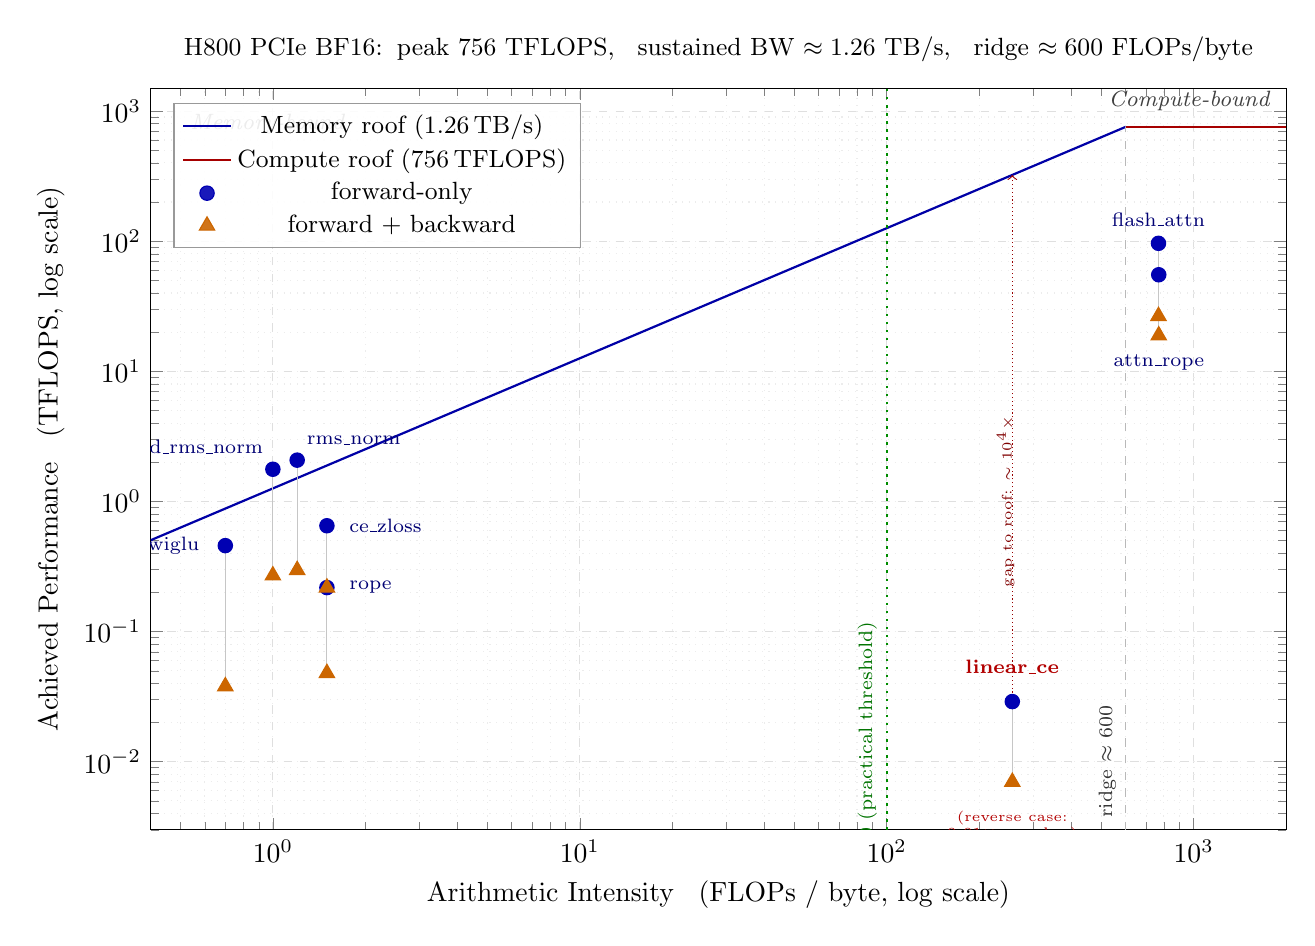
\begin{tikzpicture}
\begin{axis}[
    width=16cm,
    height=11cm,
    xmode=log, ymode=log,
    log basis x=10, log basis y=10,
    xmin=0.4, xmax=2000,
    ymin=0.003, ymax=1500,
    xlabel={Arithmetic Intensity \;\;(FLOPs / byte, log scale)},
    ylabel={Achieved Performance \;\;(TFLOPS, log scale)},
    grid=both,
    major grid style={dashed, gray!25},
    minor grid style={dotted, gray!15},
    legend style={
        at={(0.02,0.98)}, anchor=north west,
        font=\small, draw=black!40, fill=white, fill opacity=0.9,
        text opacity=1
    },
    title style={font=\small},
    title={H800 PCIe BF16:\;\;peak $756$ TFLOPS,\;\; sustained BW $\approx 1.26$ TB/s,\;\; ridge $\approx 600$ FLOPs/byte},
]

% =========================================================
% Roofline ceilings
% =========================================================
% Memory roof: P = BW * AI = 1.26 * x (TFLOPS = TB/s * FLOPs/byte)
% draws from x=0.4 up to ridge x=600, where y = 1.26*600 = 756
\addplot[thick, blue!65!black, no markers, domain=0.4:600, samples=2] {1.26*x};
\addlegendentry{Memory roof ($1.26\,$TB/s)}

% Compute roof: P = 756 TFLOPS (constant), from x=600 onward
\addplot[thick, red!65!black, no markers, domain=600:2000, samples=2] {756};
\addlegendentry{Compute roof ($756\,$TFLOPS)}

% Ridge marker (vertical dashed at AI=600)
\draw[gray!55, dashed, line width=0.5pt]
    (axis cs:600,0.003) -- (axis cs:600,756);
\node[font=\scriptsize, gray!40!black, rotate=90, anchor=south]
    at (axis cs:600,0.01) {ridge $\approx 600$};

% Practical memory-bound threshold (md: AI < 100)
\draw[green!55!black, dotted, line width=0.9pt]
    (axis cs:100,0.003) -- (axis cs:100,1500);
\node[font=\scriptsize, green!45!black, rotate=90, anchor=south]
    at (axis cs:100,0.01) {AI=100 (practical threshold)};

% =========================================================
% Per-kernel pair connecting lines (fwd <-> fwd+bwd)
% 表明 backward 的性能衰减幅度
% =========================================================
\draw[gray!45, line width=0.4pt] (axis cs:1.2, 2.079) -- (axis cs:1.2, 0.297);   % rms_norm
\draw[gray!45, line width=0.4pt] (axis cs:1.5, 0.651) -- (axis cs:1.5, 0.048);   % ce_zloss
\draw[gray!45, line width=0.4pt] (axis cs:0.7, 0.458) -- (axis cs:0.7, 0.038);   % swiglu
% rope: fwd 与 fwd+bwd TFLOPS 相同 (0.218), 不画线
\draw[gray!45, line width=0.4pt] (axis cs:1.0, 1.769) -- (axis cs:1.0, 0.270);   % add_rms_norm
\draw[gray!45, line width=0.4pt] (axis cs:768, 96.346) -- (axis cs:768, 26.588); % flash_attn
\draw[gray!45, line width=0.4pt] (axis cs:769.5, 55.256) -- (axis cs:769.5, 18.889); % attn_rope
\draw[gray!45, line width=0.4pt] (axis cs:256.5, 0.029) -- (axis cs:256.5, 0.007);   % linear_ce

% =========================================================
% Forward-only data (blue circles)
% =========================================================
\addplot[only marks, mark=*, mark size=2.6pt, blue!70!black]
    coordinates {
        (1.2, 2.079)
        (1.5, 0.651)
        (0.7, 0.458)
        (1.5, 0.218)
        (1.0, 1.769)
        (768, 96.346)
        (769.5, 55.256)
        (256.5, 0.029)
    };
\addlegendentry{forward-only}

% =========================================================
% Forward + backward data (orange triangles)
% =========================================================
\addplot[only marks, mark=triangle*, mark size=3.2pt, orange!80!black]
    coordinates {
        (1.2, 0.297)
        (1.5, 0.048)
        (0.7, 0.038)
        (1.5, 0.218)
        (1.0, 0.270)
        (768, 26.588)
        (769.5, 18.889)
        (256.5, 0.007)
    };
\addlegendentry{forward + backward}

% =========================================================
% Kernel name labels (位置经过手工调整以避免重叠)
% =========================================================
% 左下 memory-bound 簇 (5 个 kernel 挤在 AI=0.7-1.5)
\node[font=\scriptsize, blue!45!black, anchor=south west]
    at (axis cs:1.2, 2.3) {rms\_norm};
\node[font=\scriptsize, blue!45!black, anchor=south east]
    at (axis cs:1.0, 1.95) {add\_rms\_norm};
\node[font=\scriptsize, blue!45!black, anchor=west]
    at (axis cs:1.65, 0.651) {ce\_zloss};
\node[font=\scriptsize, blue!45!black, anchor=east]
    at (axis cs:0.62, 0.458) {swiglu};
\node[font=\scriptsize, blue!45!black, anchor=west]
    at (axis cs:1.65, 0.218) {rope};

% 右上 compute-bound 簇
\node[font=\scriptsize, blue!45!black, anchor=south]
    at (axis cs:768, 110) {flash\_attn};
\node[font=\scriptsize, blue!45!black, anchor=north]
    at (axis cs:769.5, 16) {attn\_rope};

% 反面案例 linear_ce — 红色突出
\node[font=\scriptsize\bfseries, red!70!black, anchor=south]
    at (axis cs:256.5, 0.04) {linear\_ce};
\node[font=\tiny, red!70!black, anchor=north, align=center]
    at (axis cs:256.5, 0.005) {(reverse case:\\$0.01\times$ speedup)};

% =========================================================
% Region annotations
% =========================================================
\node[font=\footnotesize\itshape, gray!50!black, anchor=west]
    at (axis cs:0.5, 800) {Memory-bound};
\node[font=\footnotesize\itshape, gray!50!black, anchor=east]
    at (axis cs:1900, 1200) {Compute-bound};

% =========================================================
% 关键诊断标注: linear_ce 离 compute roof 多远
% =========================================================
\draw[<->, red!60!black, line width=0.4pt, densely dotted]
    (axis cs:256.5, 0.029) -- (axis cs:256.5, 323.0);
\node[font=\tiny, red!50!black, rotate=90, anchor=south, align=center]
    at (axis cs:280, 1.0)
    {gap to roof: $\sim10^4\times$};

\end{axis}
\end{tikzpicture}
\end{document}

%
% 数据来源:
%   profile_v2_h800.md   (forward-only)        — Roofline 段 + Actual TFLOPS 列
%   profile_bwd_h800.md  (forward + backward)  — Roofline 段 + Actual TFLOPS 列
% 测试硬件: NVIDIA H800 PCIe
%   - BF16 Tensor Core peak: 756 TFLOPS (dense, 厂商标称)
%   - HBM3 sustained BW    : ~1.26 TB/s (~63% of 2.0 TB/s theoretical)
%   - Ridge point          : 756 / 1.26 ≈ 600 FLOPs/byte
%
% 设计要点:
%   - log-log 双对数: AI 跨 0.7-770 (3 数量级), TFLOPS 跨 0.007-96 (4 数量级)
%   - Memory roof (蓝色斜线, slope=BW): y = 1.26 * x, 适用于 x < 600
%   - Compute roof (红色水平线): y = 756, 适用于 x ≥ 600
%   - Ridge 灰色虚线: AI = 600 处屋脊
%   - AI=100 绿色点线: md 经验阈值 (memory-bound 实用判定)
%   - 8 kernels × 2 workloads: 蓝圆 = forward-only, 橙三角 = forward+backward
%   - 同 kernel 的 fwd / fwd+bwd 用细灰线连接, 线长直观显示 backward 性能衰减
%   - 关键 kernel 名称直接标注在点旁; 反面案例 linear_ce 突出标红
\documentclass[tikz,border=10pt]{standalone}
\usepackage{pgfplots}
\usepackage{amsmath}
\pgfplotsset{compat=1.18}

\begin{document}
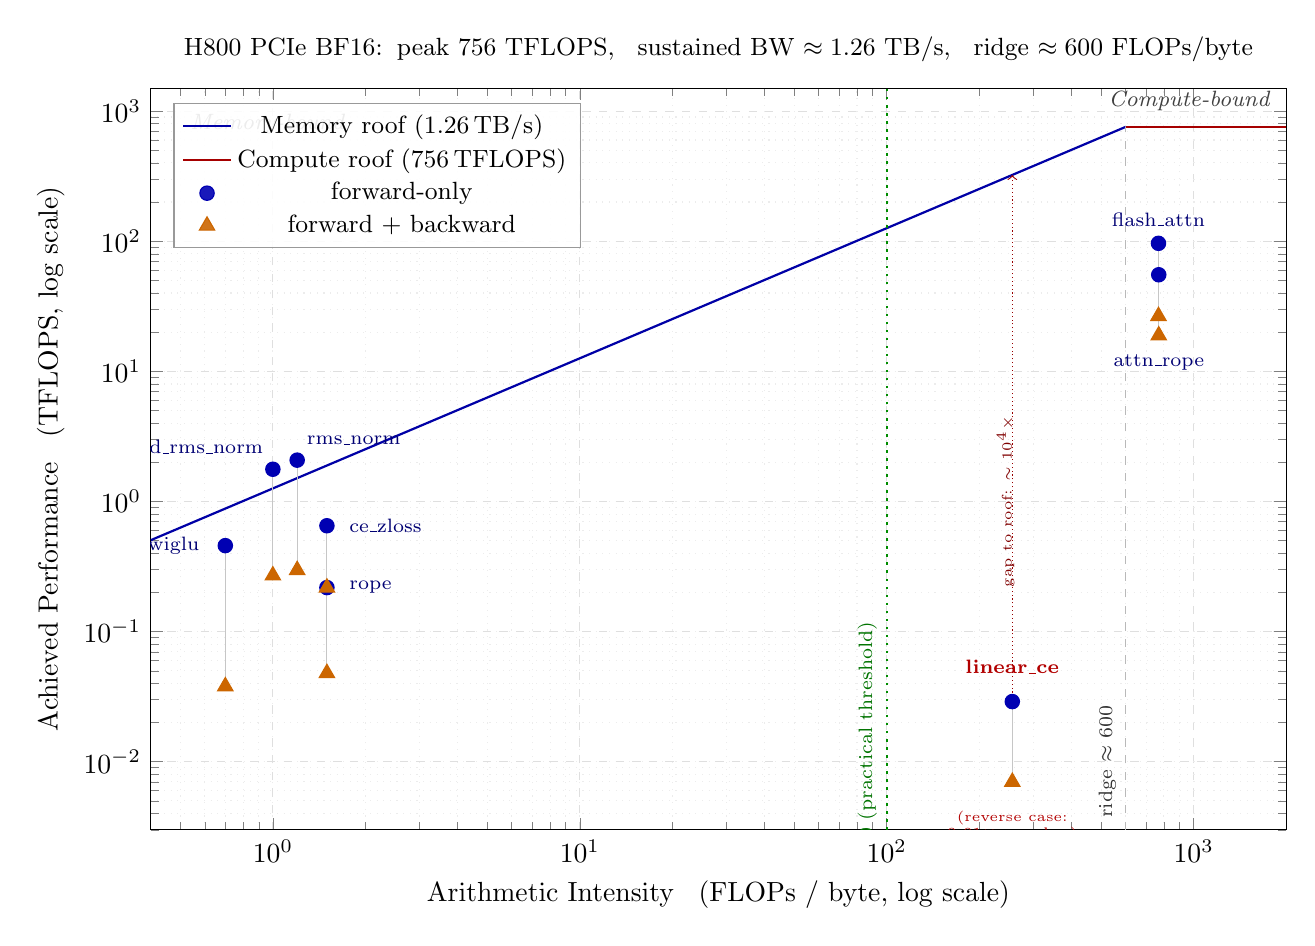
\begin{tikzpicture}
\begin{axis}[
    width=16cm,
    height=11cm,
    xmode=log, ymode=log,
    log basis x=10, log basis y=10,
    xmin=0.4, xmax=2000,
    ymin=0.003, ymax=1500,
    xlabel={Arithmetic Intensity \;\;(FLOPs / byte, log scale)},
    ylabel={Achieved Performance \;\;(TFLOPS, log scale)},
    grid=both,
    major grid style={dashed, gray!25},
    minor grid style={dotted, gray!15},
    legend style={
        at={(0.02,0.98)}, anchor=north west,
        font=\small, draw=black!40, fill=white, fill opacity=0.9,
        text opacity=1
    },
    title style={font=\small},
    title={H800 PCIe BF16:\;\;peak $756$ TFLOPS,\;\; sustained BW $\approx 1.26$ TB/s,\;\; ridge $\approx 600$ FLOPs/byte},
]

% =========================================================
% Roofline ceilings
% =========================================================
% Memory roof: P = BW * AI = 1.26 * x (TFLOPS = TB/s * FLOPs/byte)
% draws from x=0.4 up to ridge x=600, where y = 1.26*600 = 756
\addplot[thick, blue!65!black, no markers, domain=0.4:600, samples=2] {1.26*x};
\addlegendentry{Memory roof ($1.26\,$TB/s)}

% Compute roof: P = 756 TFLOPS (constant), from x=600 onward
\addplot[thick, red!65!black, no markers, domain=600:2000, samples=2] {756};
\addlegendentry{Compute roof ($756\,$TFLOPS)}

% Ridge marker (vertical dashed at AI=600)
\draw[gray!55, dashed, line width=0.5pt]
    (axis cs:600,0.003) -- (axis cs:600,756);
\node[font=\scriptsize, gray!40!black, rotate=90, anchor=south]
    at (axis cs:600,0.01) {ridge $\approx 600$};

% Practical memory-bound threshold (md: AI < 100)
\draw[green!55!black, dotted, line width=0.9pt]
    (axis cs:100,0.003) -- (axis cs:100,1500);
\node[font=\scriptsize, green!45!black, rotate=90, anchor=south]
    at (axis cs:100,0.01) {AI=100 (practical threshold)};

% =========================================================
% Per-kernel pair connecting lines (fwd <-> fwd+bwd)
% 表明 backward 的性能衰减幅度
% =========================================================
\draw[gray!45, line width=0.4pt] (axis cs:1.2, 2.079) -- (axis cs:1.2, 0.297);   % rms_norm
\draw[gray!45, line width=0.4pt] (axis cs:1.5, 0.651) -- (axis cs:1.5, 0.048);   % ce_zloss
\draw[gray!45, line width=0.4pt] (axis cs:0.7, 0.458) -- (axis cs:0.7, 0.038);   % swiglu
% rope: fwd 与 fwd+bwd TFLOPS 相同 (0.218), 不画线
\draw[gray!45, line width=0.4pt] (axis cs:1.0, 1.769) -- (axis cs:1.0, 0.270);   % add_rms_norm
\draw[gray!45, line width=0.4pt] (axis cs:768, 96.346) -- (axis cs:768, 26.588); % flash_attn
\draw[gray!45, line width=0.4pt] (axis cs:769.5, 55.256) -- (axis cs:769.5, 18.889); % attn_rope
\draw[gray!45, line width=0.4pt] (axis cs:256.5, 0.029) -- (axis cs:256.5, 0.007);   % linear_ce

% =========================================================
% Forward-only data (blue circles)
% =========================================================
\addplot[only marks, mark=*, mark size=2.6pt, blue!70!black]
    coordinates {
        (1.2, 2.079)
        (1.5, 0.651)
        (0.7, 0.458)
        (1.5, 0.218)
        (1.0, 1.769)
        (768, 96.346)
        (769.5, 55.256)
        (256.5, 0.029)
    };
\addlegendentry{forward-only}

% =========================================================
% Forward + backward data (orange triangles)
% =========================================================
\addplot[only marks, mark=triangle*, mark size=3.2pt, orange!80!black]
    coordinates {
        (1.2, 0.297)
        (1.5, 0.048)
        (0.7, 0.038)
        (1.5, 0.218)
        (1.0, 0.270)
        (768, 26.588)
        (769.5, 18.889)
        (256.5, 0.007)
    };
\addlegendentry{forward + backward}

% =========================================================
% Kernel name labels (位置经过手工调整以避免重叠)
% =========================================================
% 左下 memory-bound 簇 (5 个 kernel 挤在 AI=0.7-1.5)
\node[font=\scriptsize, blue!45!black, anchor=south west]
    at (axis cs:1.2, 2.3) {rms\_norm};
\node[font=\scriptsize, blue!45!black, anchor=south east]
    at (axis cs:1.0, 1.95) {add\_rms\_norm};
\node[font=\scriptsize, blue!45!black, anchor=west]
    at (axis cs:1.65, 0.651) {ce\_zloss};
\node[font=\scriptsize, blue!45!black, anchor=east]
    at (axis cs:0.62, 0.458) {swiglu};
\node[font=\scriptsize, blue!45!black, anchor=west]
    at (axis cs:1.65, 0.218) {rope};

% 右上 compute-bound 簇
\node[font=\scriptsize, blue!45!black, anchor=south]
    at (axis cs:768, 110) {flash\_attn};
\node[font=\scriptsize, blue!45!black, anchor=north]
    at (axis cs:769.5, 16) {attn\_rope};

% 反面案例 linear_ce — 红色突出
\node[font=\scriptsize\bfseries, red!70!black, anchor=south]
    at (axis cs:256.5, 0.04) {linear\_ce};
\node[font=\tiny, red!70!black, anchor=north, align=center]
    at (axis cs:256.5, 0.005) {(reverse case:\\$0.01\times$ speedup)};

% =========================================================
% Region annotations
% =========================================================
\node[font=\footnotesize\itshape, gray!50!black, anchor=west]
    at (axis cs:0.5, 800) {Memory-bound};
\node[font=\footnotesize\itshape, gray!50!black, anchor=east]
    at (axis cs:1900, 1200) {Compute-bound};

% =========================================================
% 关键诊断标注: linear_ce 离 compute roof 多远
% =========================================================
\draw[<->, red!60!black, line width=0.4pt, densely dotted]
    (axis cs:256.5, 0.029) -- (axis cs:256.5, 323.0);
\node[font=\tiny, red!50!black, rotate=90, anchor=south, align=center]
    at (axis cs:280, 1.0)
    {gap to roof: $\sim10^4\times$};

\end{axis}
\end{tikzpicture}
\end{document}

%
% 数据来源:
%   profile_v2_h800.md   (forward-only)        — Roofline 段 + Actual TFLOPS 列
%   profile_bwd_h800.md  (forward + backward)  — Roofline 段 + Actual TFLOPS 列
% 测试硬件: NVIDIA H800 PCIe
%   - BF16 Tensor Core peak: 756 TFLOPS (dense, 厂商标称)
%   - HBM3 sustained BW    : ~1.26 TB/s (~63% of 2.0 TB/s theoretical)
%   - Ridge point          : 756 / 1.26 ≈ 600 FLOPs/byte
%
% 设计要点:
%   - log-log 双对数: AI 跨 0.7-770 (3 数量级), TFLOPS 跨 0.007-96 (4 数量级)
%   - Memory roof (蓝色斜线, slope=BW): y = 1.26 * x, 适用于 x < 600
%   - Compute roof (红色水平线): y = 756, 适用于 x ≥ 600
%   - Ridge 灰色虚线: AI = 600 处屋脊
%   - AI=100 绿色点线: md 经验阈值 (memory-bound 实用判定)
%   - 8 kernels × 2 workloads: 蓝圆 = forward-only, 橙三角 = forward+backward
%   - 同 kernel 的 fwd / fwd+bwd 用细灰线连接, 线长直观显示 backward 性能衰减
%   - 关键 kernel 名称直接标注在点旁; 反面案例 linear_ce 突出标红
\documentclass[tikz,border=10pt]{standalone}
\usepackage{pgfplots}
\usepackage{amsmath}
\pgfplotsset{compat=1.18}

\begin{document}
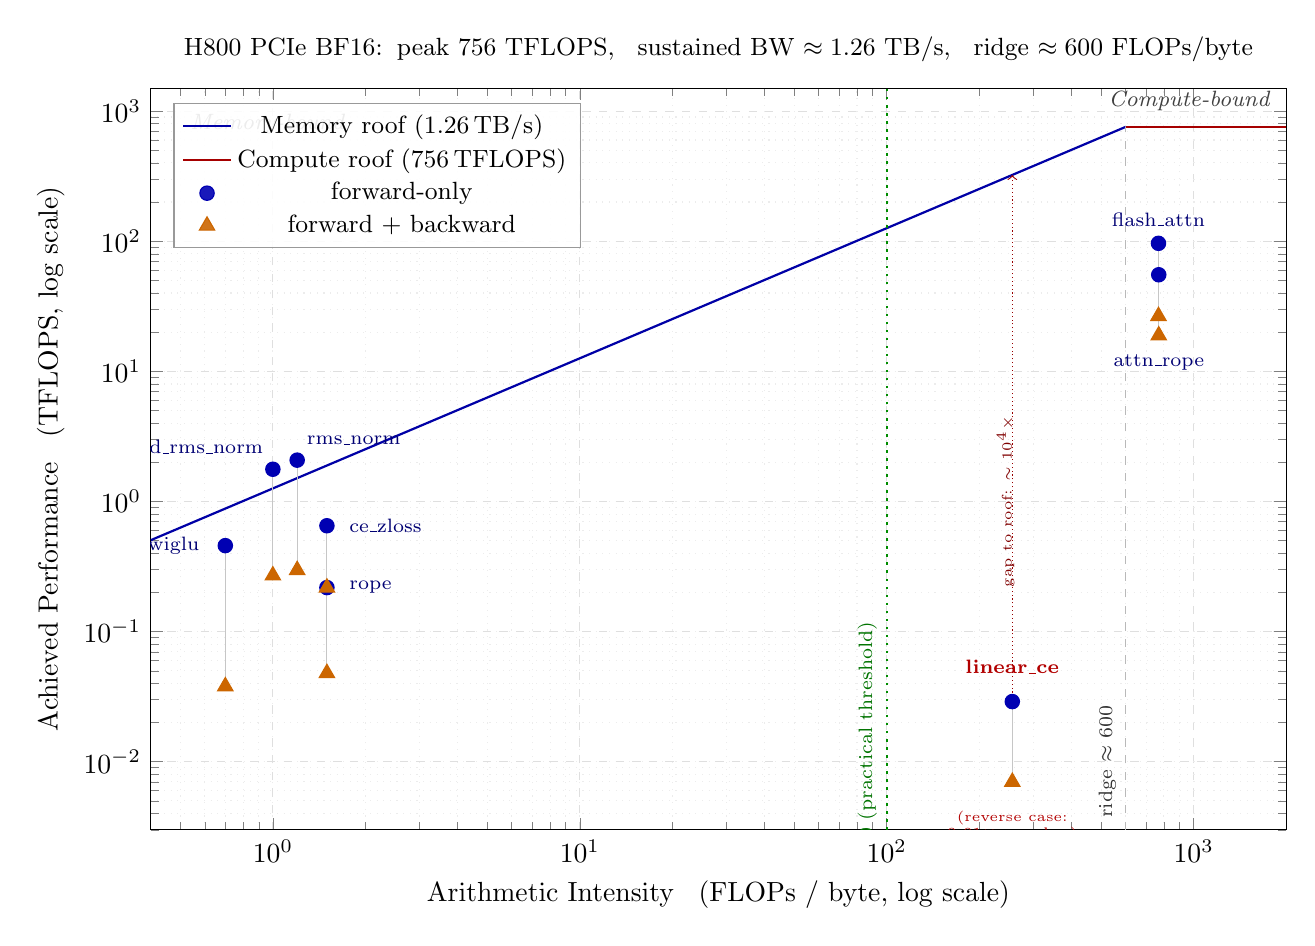
\begin{tikzpicture}
\begin{axis}[
    width=16cm,
    height=11cm,
    xmode=log, ymode=log,
    log basis x=10, log basis y=10,
    xmin=0.4, xmax=2000,
    ymin=0.003, ymax=1500,
    xlabel={Arithmetic Intensity \;\;(FLOPs / byte, log scale)},
    ylabel={Achieved Performance \;\;(TFLOPS, log scale)},
    grid=both,
    major grid style={dashed, gray!25},
    minor grid style={dotted, gray!15},
    legend style={
        at={(0.02,0.98)}, anchor=north west,
        font=\small, draw=black!40, fill=white, fill opacity=0.9,
        text opacity=1
    },
    title style={font=\small},
    title={H800 PCIe BF16:\;\;peak $756$ TFLOPS,\;\; sustained BW $\approx 1.26$ TB/s,\;\; ridge $\approx 600$ FLOPs/byte},
]

% =========================================================
% Roofline ceilings
% =========================================================
% Memory roof: P = BW * AI = 1.26 * x (TFLOPS = TB/s * FLOPs/byte)
% draws from x=0.4 up to ridge x=600, where y = 1.26*600 = 756
\addplot[thick, blue!65!black, no markers, domain=0.4:600, samples=2] {1.26*x};
\addlegendentry{Memory roof ($1.26\,$TB/s)}

% Compute roof: P = 756 TFLOPS (constant), from x=600 onward
\addplot[thick, red!65!black, no markers, domain=600:2000, samples=2] {756};
\addlegendentry{Compute roof ($756\,$TFLOPS)}

% Ridge marker (vertical dashed at AI=600)
\draw[gray!55, dashed, line width=0.5pt]
    (axis cs:600,0.003) -- (axis cs:600,756);
\node[font=\scriptsize, gray!40!black, rotate=90, anchor=south]
    at (axis cs:600,0.01) {ridge $\approx 600$};

% Practical memory-bound threshold (md: AI < 100)
\draw[green!55!black, dotted, line width=0.9pt]
    (axis cs:100,0.003) -- (axis cs:100,1500);
\node[font=\scriptsize, green!45!black, rotate=90, anchor=south]
    at (axis cs:100,0.01) {AI=100 (practical threshold)};

% =========================================================
% Per-kernel pair connecting lines (fwd <-> fwd+bwd)
% 表明 backward 的性能衰减幅度
% =========================================================
\draw[gray!45, line width=0.4pt] (axis cs:1.2, 2.079) -- (axis cs:1.2, 0.297);   % rms_norm
\draw[gray!45, line width=0.4pt] (axis cs:1.5, 0.651) -- (axis cs:1.5, 0.048);   % ce_zloss
\draw[gray!45, line width=0.4pt] (axis cs:0.7, 0.458) -- (axis cs:0.7, 0.038);   % swiglu
% rope: fwd 与 fwd+bwd TFLOPS 相同 (0.218), 不画线
\draw[gray!45, line width=0.4pt] (axis cs:1.0, 1.769) -- (axis cs:1.0, 0.270);   % add_rms_norm
\draw[gray!45, line width=0.4pt] (axis cs:768, 96.346) -- (axis cs:768, 26.588); % flash_attn
\draw[gray!45, line width=0.4pt] (axis cs:769.5, 55.256) -- (axis cs:769.5, 18.889); % attn_rope
\draw[gray!45, line width=0.4pt] (axis cs:256.5, 0.029) -- (axis cs:256.5, 0.007);   % linear_ce

% =========================================================
% Forward-only data (blue circles)
% =========================================================
\addplot[only marks, mark=*, mark size=2.6pt, blue!70!black]
    coordinates {
        (1.2, 2.079)
        (1.5, 0.651)
        (0.7, 0.458)
        (1.5, 0.218)
        (1.0, 1.769)
        (768, 96.346)
        (769.5, 55.256)
        (256.5, 0.029)
    };
\addlegendentry{forward-only}

% =========================================================
% Forward + backward data (orange triangles)
% =========================================================
\addplot[only marks, mark=triangle*, mark size=3.2pt, orange!80!black]
    coordinates {
        (1.2, 0.297)
        (1.5, 0.048)
        (0.7, 0.038)
        (1.5, 0.218)
        (1.0, 0.270)
        (768, 26.588)
        (769.5, 18.889)
        (256.5, 0.007)
    };
\addlegendentry{forward + backward}

% =========================================================
% Kernel name labels (位置经过手工调整以避免重叠)
% =========================================================
% 左下 memory-bound 簇 (5 个 kernel 挤在 AI=0.7-1.5)
\node[font=\scriptsize, blue!45!black, anchor=south west]
    at (axis cs:1.2, 2.3) {rms\_norm};
\node[font=\scriptsize, blue!45!black, anchor=south east]
    at (axis cs:1.0, 1.95) {add\_rms\_norm};
\node[font=\scriptsize, blue!45!black, anchor=west]
    at (axis cs:1.65, 0.651) {ce\_zloss};
\node[font=\scriptsize, blue!45!black, anchor=east]
    at (axis cs:0.62, 0.458) {swiglu};
\node[font=\scriptsize, blue!45!black, anchor=west]
    at (axis cs:1.65, 0.218) {rope};

% 右上 compute-bound 簇
\node[font=\scriptsize, blue!45!black, anchor=south]
    at (axis cs:768, 110) {flash\_attn};
\node[font=\scriptsize, blue!45!black, anchor=north]
    at (axis cs:769.5, 16) {attn\_rope};

% 反面案例 linear_ce — 红色突出
\node[font=\scriptsize\bfseries, red!70!black, anchor=south]
    at (axis cs:256.5, 0.04) {linear\_ce};
\node[font=\tiny, red!70!black, anchor=north, align=center]
    at (axis cs:256.5, 0.005) {(reverse case:\\$0.01\times$ speedup)};

% =========================================================
% Region annotations
% =========================================================
\node[font=\footnotesize\itshape, gray!50!black, anchor=west]
    at (axis cs:0.5, 800) {Memory-bound};
\node[font=\footnotesize\itshape, gray!50!black, anchor=east]
    at (axis cs:1900, 1200) {Compute-bound};

% =========================================================
% 关键诊断标注: linear_ce 离 compute roof 多远
% =========================================================
\draw[<->, red!60!black, line width=0.4pt, densely dotted]
    (axis cs:256.5, 0.029) -- (axis cs:256.5, 323.0);
\node[font=\tiny, red!50!black, rotate=90, anchor=south, align=center]
    at (axis cs:280, 1.0)
    {gap to roof: $\sim10^4\times$};

\end{axis}
\end{tikzpicture}
\end{document}
